\documentclass[tikz]{standalone}
\usetikzlibrary{calc,trees,positioning,arrows,chains,shapes.geometric,%
    decorations.pathreplacing,decorations.pathmorphing,shapes,%
    matrix,shapes.symbols,fit}

\pgfdeclarelayer{back}
\pgfsetlayers{back,main}

\begin{document}
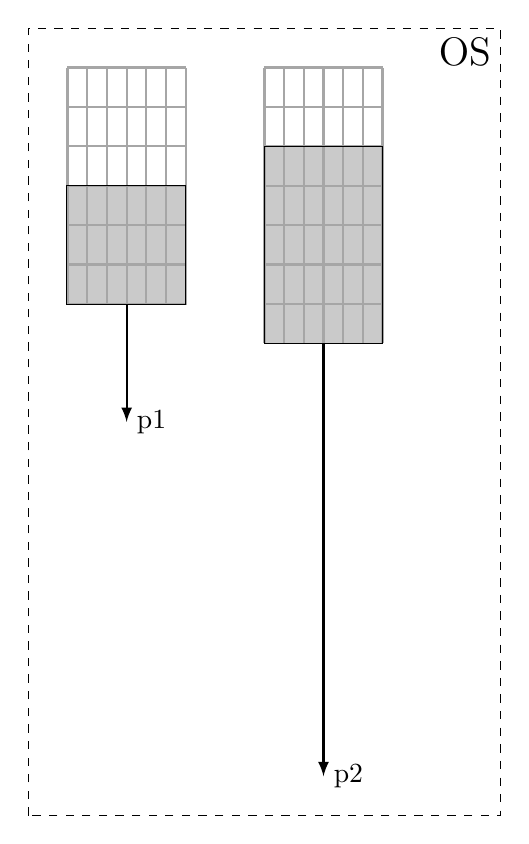
\begin{tikzpicture}

\draw[dashed] (0,0) rectangle (6,10) node[anchor=north east,font=\Large] {OS};

%process 1
\draw[thick,draw=gray!70] (.49,6.49) grid[xstep=.25cm,ystep=.5cm] (2,9.5);
\draw[thick,-latex] (1.25,6.5) -- (1.25,5) node[anchor=west] {p1};
\draw[fill=gray!70,fill opacity=.6] (.49,6.49) rectangle (2,8);

\draw[thick,draw=gray!70] (2.99,6) grid[xstep=.25cm,ystep=.5cm] (4.5,9.5);
\draw[thick,-latex] (3.75,6) -- (3.75,.5) node[anchor=west] {p2};
\draw[fill=gray!70,fill opacity=.6] (3,6) rectangle (4.5,8.5);

  \end{tikzpicture}
\end{document}
